\documentclass[a4paper, 12pt]{article}
% ----- Loading the Package MCMthesis -----
% -----           v 5.01-L            -----
% `tcn' is short for `Team Control Number'.
% You should fill your tcn after the equal sign following tcn.
% The option `sheet' contorls whether the summary sheet
% will appear.
% The option `abstract' controls whether the abstract
% will appear in the title-page.
\usepackage[tcn = 55429, sheet = true, abstract = false]{MCMthesis}
% ----- Question Mark -----
\problem{D}
% ----- Fonts settings -----
% You may need to install the font files, if it's needed.
% Disable it, if you don't want this font.
\usepackage{palatino}

%各种宏包
\usepackage{indentfirst}
\usepackage{color}
\usepackage{caption}
\usepackage{cite}
\usepackage{graphicx}
\usepackage{array}
\usepackage{float}
\usepackage{amsmath}
\usepackage{booktabs}
\usepackage{subfigure}
\usepackage{listings}
\usepackage[marginal]{footmisc}
\allowdisplaybreaks
% ----- Set the skip betweent the paragraphics -----
\setlength\parskip{.5\baselineskip}
% ----- The name of Abstract ------
\providecommand{\abstractname}{\relax} % <-- Do not modify here.
\renewcommand{\abstractname}{Summary} % <-- Modify here, if needed.


% -----------------------------------
% ===== The Title of Your Paper =====
% -----------------------------------
\title{The \LaTeX Template for  MCM Version 5.0}
% ---------------------------------------
% ===== The Author(s) of Your Paper =====
% ---------------------------------------
\author{\small \href{http://www.latexstudio.net/}{\includegraphics[width=7cm]{logo}}}
% ----------------
% ===== Time =====
% ----------------
\date{\today}
\begin{document}
\nocite{*}
\bibliographystyle{unsrt}
% Abstract should be put before `\maketitle'
%!TEX root = mcmpaper.tex
\begin{abstract}
In order to protect people's security and to provide more convenience, the reasonable setting of the airport security procedures is of great importance. This paper take the airport security inspection process as the main research object and use relevant theory, through the establishment and analysis of the model to find the bottlenecks in the current security inspection process and optimize the security system to get the best solution. And this paper also consider the influence of cultural differences and give some reasonable suggestions.\\
To establish the initial model, this paper first analyze the information given by the subject, and make reasonable assumptions. This paper use the queuing theory model to describe the queueing situation. And we transform the real airport security inspection system to a Petri net to simplify calculation. Then this paper use programming method to simulate the flow of passengers between various zones through computer simulation and give out the average passing time and its standard deviation on the chart, it's obvious that Zone A and B are the bottlenecks in the security process.\\
To optimizing the bottlenecks, this paper establish a evaluation index system including queuing satisfaction and cost effect. Firstly, we can increase the personnel and equipment in Zone A and B, but the values can not increase without limit considering the cost of modifications. Therefore, by this system, we can find out values that can not only greatly optimize the wait time but also save money. The result show that 11 officers in Zone A and 24 sets of equipment in Zone B will be the best program which can save over 50\% time. Besides, we can adjust the procedures, for the most crowded and time consuming Zone B, we can moderately increase the officer to sharply reduce the congestion of passengers and improve the travel experience.
\\
In order to find out the effect of different cultures, two culture differences are mentioned as analysis object. This paper quantified the influence and then change the corresponding parameter in the simulation program to get the result to make sensitivity analysis. And proposes are also given to accommodate these differences. For example, more equipment should be offered in places with more belongings.

\end{abstract}


\pagestyle{fancy}
\maketitle


\newpage
% Generate the Table of Contents, if it's needed.
\tableofcontents
\newpage
% The body of your paper
%!TEX root = mcmpaper.tex

\newcommand\degree{^{\circ}}

%1 问题重述
%!TEX root = mcmpaper.tex

%======================问题重述====================================
\section{Problems restatement}

\subsection{Introduction}
Following the terrorist attacks in the US on September 11,2001, airport security has been significantly enhanced throughout the world, the security situation has also been improved. In order to ensure the safety of all passengers, every passenger must pass the security checkpoint before entering the airport, but a lot of inconvenience is also caused. How to maximize security while minimizing inconvenience to passengers, the research of this problem is of great significance in the present air traffic business.

\subsection{Restatement}
The flow of US airport security checkpoints is known as followed: First line up to check the identification and board documents in Zone A, then check the body and belongings in Zone B, then collect belongings in Zone C, if there's nothing wrong, then you can leave. Passengers that fail this step receive a pat-down inspection in Zone D.
Besides, approximately 45\% of passengers enroll in a program called Pre-Check for trusted travelers, these passengers pay 85\$ to receive a background check and enjoy a separate screening process for five years, in this way they can save some time in Zone B. Data of time in each step has been offered.
\par
Our tasks are:
\begin{enumerate}
  \item Establish a reasonable model to identify bottlenecks.
  \item Develop two or more potential modifications to the current process to improve passenger throughput and reduce variance in wait time.
  \item Consider cultural differences and analyze how can the security system accommodate these differences.
  \item Propose policy and procedural recommendations for the security managers based on the model.
\end{enumerate}


%2 问题分析
%!TEX root = mcmpaper.tex
\section{Model Analysis}
\subsection{Analysis of problem a}
% 第一问分析
As we are aware of the detailed process of security check and data of each step, we can get the time every passenger spent in each Zone of the security checkpoint. After making reasonable assumption, we can simulate out the average wait time and variance in wait time of passengers in the security checkpoint by computer programming. To establish the Model 1 and identify the bottlenecks and problematic Zones.
\subsection{Analysis of problem b}
% 第二问分析
Based on the Model 1, we should develop modifications to improve passenger throughput and reduce variance in wait time. Firstly we set the Zone A for both Pre-check and regular check to use, then we adjust the number of officers in Zone A and Pre-check and regular lanes in Zone B. Because the bottleneck has been identified in Model 1, through traversal adjustment to the number of lanes in a certain range, we can get the passenger throughput and wait time variance in each condition. Considering the cost, we should choose the best number of Zone A officer and lanes in Zone B. In addition, the details of the process can also be changed such as adding another security officer next to the belt in Zone B to slow down the blockage of manual check.

\subsection{Analysis of problem c}
% 第三问分析
In this problem we consider how cultural differences may impact the way in which passenger's process through checkpoints as a sensitivity analysis. We take two cultural differences into consideration. One is passengers in some places are much slower, which will result in a longer time of the whole process. The other is that in some area like Italy people enjoy chic lifestyle and wouldn't like to take much belongings, so the time in Zone B will reduce. We take these two differences into simulation separately and make sensitivity analysis.


%3 模型假设
%!TEX root = mcmpaper.tex

%======================Model Assumptions====================================
\section{Model Assumptions}
The model should be based on the six following assumptions:
\begin{itemize}
  \item Assumption 1:The passengers are slower than belongings: This is based on our life experience.
  \item Assumption 2:Develop two or more potential modifications to the current process to improve passenger throughput and reduce variance in wait time.
  \item Assumption 3:The number of passengers to the airport is 75000: We take Chicago O'Hare Airport as an example, and we find the passenger traffic in the related news.
  \item Assumption 4:The time required for the officer to perform security checks is normally distributed.
  \item Assumption 5:There is not any emergency event happened in airport.
  \item Assumption 6:Passengers with Pre-check qualification are all queued at the Pre-check lanes.
\end{itemize}


%4 符号申明
%!TEX root = mcmpaper.tex

%==================================符号声明========================================
\section{Notations}
\begin{table}[H]
\centering
\caption{Notations}\label{tab:notations}
\begin{tabular}{|c|c|c|}
\hline
Notations& Definition& Dimension\\ \hline
$P_{i}$& The probability of an event & None \\
\hline
$T_{i}$& The elapsed time of an event & s \\\hline
P & Queuing satisfaction & None \\\hline
L & The time required to pass all security checks & s \\\hline
S & The standard deviation of the security period & s \\\hline
C & Cost effect & None \\\hline
$A_{0}$ & The initial state of the equipment personnel in Zone A & set \\\hline
$A_{t}$ & Improved zone A equipment personnel & set \\\hline
$B_{0}$ & The initial state of the equipment personnel in Zone B & set \\\hline
$B_{t}$ & Improved zone B equipment personnel & set \\
\hline
\end{tabular}
\end{table}

%4 问题一模型建立与求解
%!TEX root = mcmpaper.tex

%===============================模型设计============================================
\section{Problem a model design}
\subsection{The distribution of tourists}
The distribution of passengers into the airport is as followed:
\par
According to the assumption 2, passengers arrive at Poisson flow. The probability of the total number of passengers arriving at the airport in time t is as followed:

% \begin{equation}
% \left.
% \begin{aligned}[b]
%   f(x)=\frac{1}{\sqrt{2\pi }*3.7926}*e^{-\frac{(x-11.2125)^2}{2*14.384}}
% \end{aligned}
% \right.
% \end{equation}

\begin{equation}
\left.
\begin{aligned}[b]
	{P_{n}}(t)=\frac{(\lambda t)^{n}}{n!}*e^{-\lambda t}
\end{aligned}
\right.
\end{equation}

parameter $\lambda$ is the average number of the passengers arrive at unit time. According to 24 hours a day, the total passenger flow is 75000, we calculate out $\lambda$=0.8681 p/s.

\begin{equation}
\left.
\begin{aligned}[b]
	{P_{n}}(t)=\frac{(0.8681t)^{n}}{n!}*e^{-0.8681t}
\end{aligned}
\right.
\end{equation}

the time interval between any two passengers meet the negative exponential distribution $\lambda$=0.8681 p/s, the Distribution function:

\begin{equation}
\left.
\begin{aligned}[b]
	F(t)=1-e^{-0.8681t}~ ~t\geq 0
\end{aligned}
\right.
\end{equation}

Set $R=F(t)$, therefore R is evenly distributed in (0,1). Through inverse transformation we get:

\begin{equation}
\left.
\begin{aligned}
	T=-\frac{1}{0.8681}ln(1-R)=-1.1519ln(1-R)
\end{aligned}
\right.
\end{equation}

Set $U=1-R$,and $U$ is also evenly distributed in $(0,1)$. The time interval $T$ between any two passengers is a random number subject to exponential distribution:

\begin{equation}
\left.
\begin{aligned}
	T=-1.1519ln U
\end{aligned}
\right.
\end{equation}

\subsection{The security process}
According to the assumptions and data offered in the Excel, we can draw a airport security Petri Net Model as followed:

\subsubsection*{Petri Net}
Petri Net is an effective model tool to describe and analyze the system with concurrent and synchronous features. We consider the security check as a system, which is synchronized and concurrent. Using time parameter based on the actual situation to analyze the time of model. Then choose the Generalized Stochastic Petri Net, GSPN to modeling the security check process.

\begin{figure}[H]
\centering
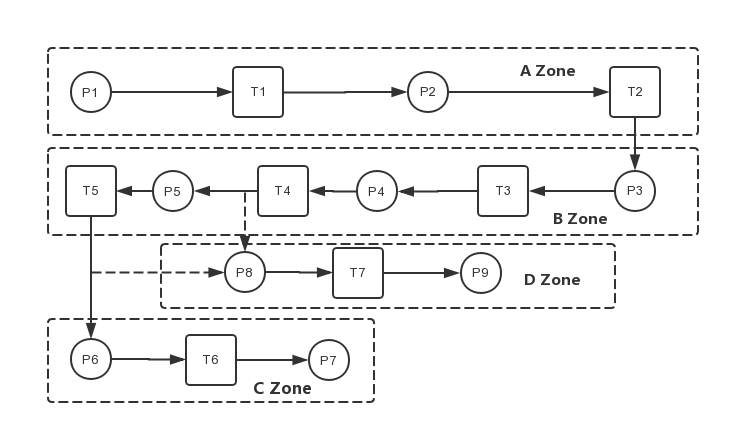
\includegraphics[width=17cm,height=12cm]{/Pic/patrymodel.png}
\caption{Petri network diagram}\label{fig:Petri_Pic}
\end{figure}



\subsubsection*{Symbols in the picture}
\begin{table}[H]
\centering
\caption{Notations}\label{tab:notations}
\begin{tabular}{|c|c|}
\hline
Symbol& Meaning\\
$P_{1}$& Arrivals at the airport \\
\hline
$P_{2}$& Passengers to start receiving identity checks \\\hline
$P_{3}$& Passengers waiting in the queue in Zone B to put their belongings to screening \\\hline
$P_{4}$& Passengers starting to put their belongings on the belt\\\hline
$P_{5}$& Passengers starting to go through scanner\\\hline
$P_{6}$& Passengers packing belongings in Zone C\\\hline
$P_{7}$& Passengers finished the whole process\\\hline
$P_{8}$& Passengers failed step receive a pat-down inspection\\\hline
$P_{9}$& Passengers finished the inspection in Zone D(10\%)
\\\hline
$T_{1}$& Time of waiting for identity verification \\\hline
$T_{2}$& Time of receiving the identity verification(average 11.21s, standard deviation 3.79s) \\\hline
$T_{3}$& Time of waiting for belongings screening\\\hline
$T_{4}$& Time of putting the belongings on the belt\\\hline
$T_{5}$& Time of receiving body inspection(average 41s, standard deviation 6.9s)\\\hline
$T_{6}$& Time of passengers to pack belongings
\\\hline
$T_{7}$& Time of receiving inspection in Zone D
\\\hline

\hline
\end{tabular}
\end{table}


\subsection{Model establishment and solution}
 Based on the above information we can carry out simulation of the airport flow by computer, here are the programming method:
\par
 The entities in the simulation program are composed of passengers, zone A, zone B, zone B and zone D, the controller consists of a time controller and a passenger controller. Here are the description of the relevant attributes and logical description:
\subsubsection*{Attributes Description:}
\paragraph*{Passenger:}
\begin{enumerate}
	\item Time to reach the airport
 	\item Time to leave the security zone
 	\item Whether to buy the  background check
 	\item Time to reach the zone A
 	\item Time to leave the zone A
  	\item Time to reach the zone B
 	\item Time to leave the zone B
 	\item Time to reach the zone C
 	\item Time to leave the zone C
 	\item Time to reach the zone D
 	\item Time to leave the zone D
\end{enumerate}
\paragraph*{Zone}
\begin{enumerate}
	\item Name
	\item The waiting list
\end{enumerate}

\subsubsection*{Logical Description:}
\begin{enumerate}
	\item The time controller increase the time by one second and ask the passenger controller how many passengers reaching the airport at that second. Then the passenger controller put the coming passengers into zone A's waiting list.
	\item The time controller informs all zones to take action
	\item Zone A Reduces the processing time by one for all passengers who are checking documents, then put the passengers who complete the task without problem into zone B's waiting list. Finally, take passengers from zone A's waiting list and set their processing time.
	\item Zone B Reduces the processing time by one for all passengers who are accepting checking, then put the passengers who complete the task without problem into zone C's waiting list and put the other problematic passengers into zone D's waiting list. Finally, take passengers from zone B's waiting list and set their processing time.
	\item Zone C Reduces the processing time by one for all passengers who are packing belongings, then record the data of passengers who complete the task.Finally, delete the passengers and take passengers from zone C's waiting list and set their processing time.
	\item Zone D Reduces the processing time by one for all passengers who are accepting addtional search, then record the data of passengers who complete the task.Finally, delete the passengers and take passengers from zone D's waiting list and set their processing time.
	\item Repeat step 1,2,3,4,5 until all passengers are deleted
	\item Run the script to extract the data and analysis
\end{enumerate}


\subsubsection*{Activity Diagram:}
\begin{figure}[H]
\centering
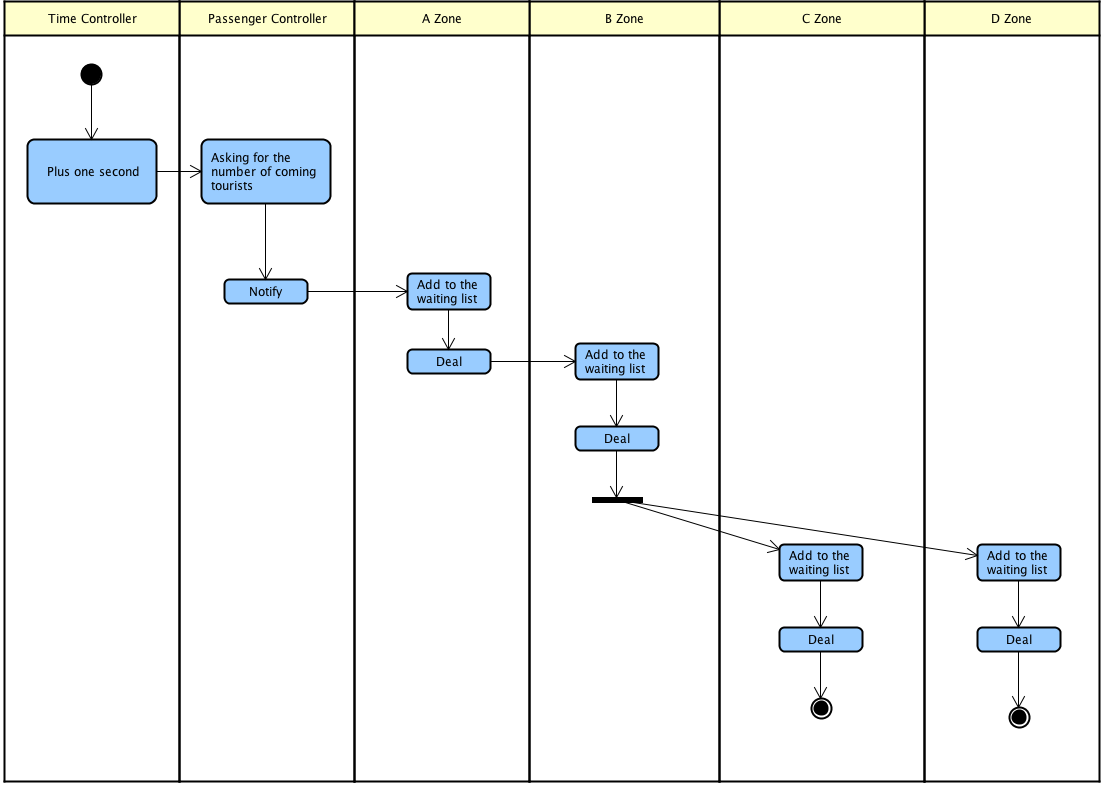
\includegraphics[width=14cm,height=8cm]{/Pic/activity_diagram.png}
\caption{Activity diagram}\label{fig:acd}
\end{figure}

\subsection{Model summary}
According to the above programming ideas for programming simulation, the average time of passengers waiting in each Zone is as followed:

\begin{figure}[H]
\centering
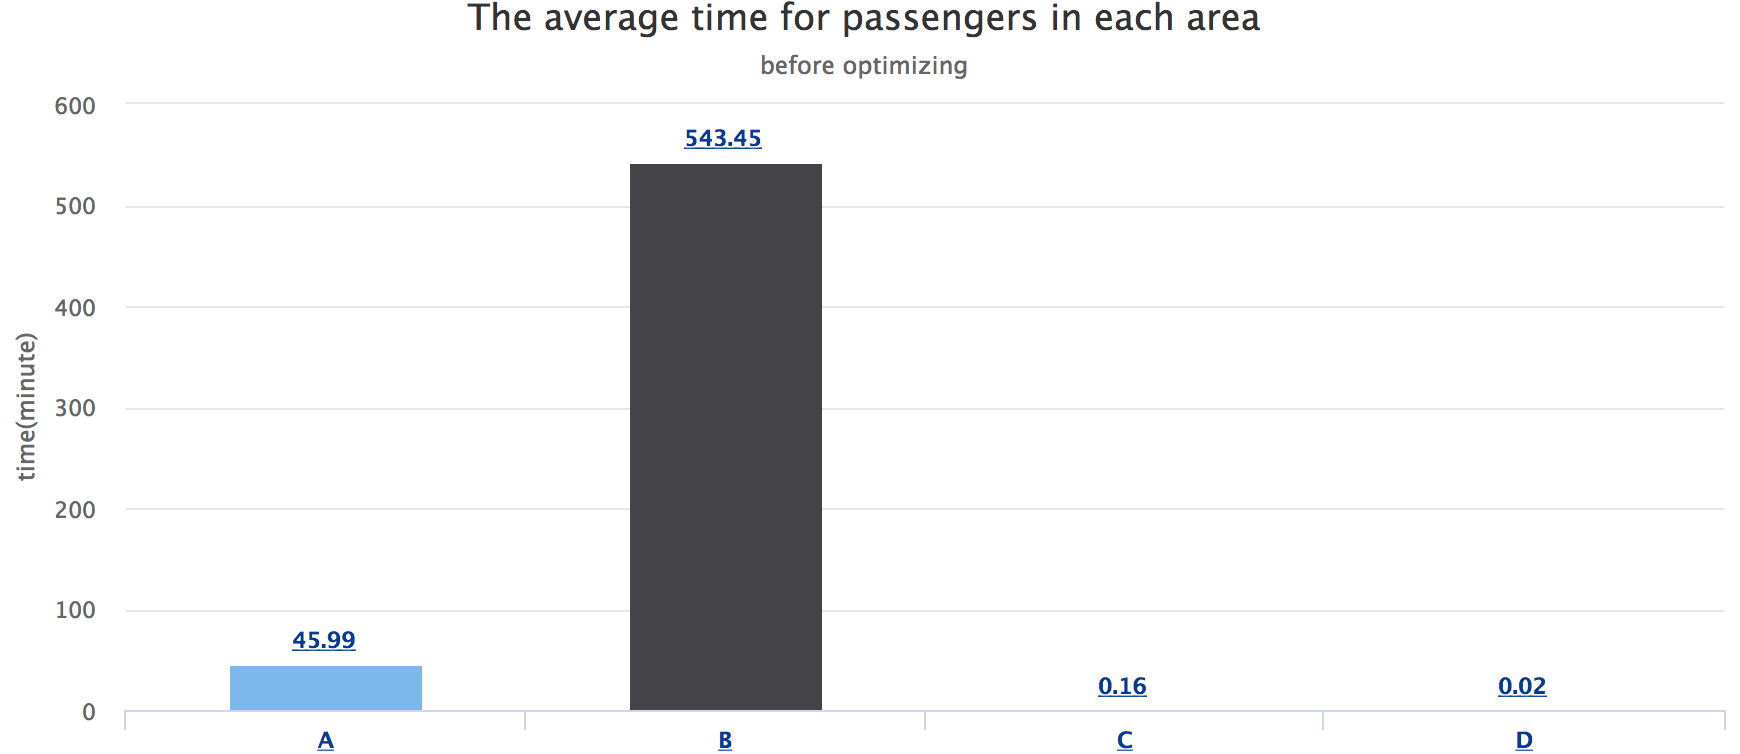
\includegraphics[width=14cm,height=8cm]{/Pic/第一问瓶颈图.png}
\caption{Bottleneck in process}\label{fig:bottleneck}
\end{figure}

We can conclude from the picture that \textbf{the time passengers spent in A and B are the most, which is hundreds times of C and D. So the bottlenecks are Zone A and B, which should be focusing optimized in our future modeling.}










%5 问题二模型建立与求解
%!TEX root = mcmpaper.tex
\section{problem b model design}
premise: In order to better measure our optimization effect, we introduce two parameters: queuing satisfaction, and cost effect.As explained below:

\begin{equation}
\left.
\begin{aligned}[b]
  P = \frac{1}{L*S}\footnotemark[1]
\end{aligned}
\right.
\end{equation}

\begin{equation}
\left.
\begin{aligned}[b]
  C=\frac{A_{t}}{A_{0}}+\frac{B_{t}}{B_{0}}
  \footnotemark[2]
\end{aligned}
\right.
\end{equation}

\footnotetext[1]{
	\textbf{P}: Queuing satisfaction\\ 
	\textbf{L}: The time required to pass all security checks;\\ 
	\textbf{S}: The standard deviation of the security period;
}

\footnotetext[2]{
	\textbf{$A_{0}$}: The initial state of the equipment personnel in zone A;\\ 
	\textbf{$A_{t}$}: Improved zone A's equipment personnel;\\ 
	\textbf{$B_{0}$}: The initial state of the equipment personnel in zone B;\\
	\textbf{$B_{t}$}: TImproved zone B's equipment personnel;
}

\subsection{Improve 1}
On the basis of Problem 1, we have recognized the bottleneck. In order to further improve the airport security throughput and reduce the waiting time difference, we first thought is to improve the security process of the zone A . As shown in the title, passengers waiting in zone A for identity verification are inspected at two locations, the travelers using the Pre-Check process and regular travelers. But for the process of identity verification, the use of Pre-Check process or not is not affected. So in order to make full use of each verification entrance of zone A, we cancel the respective queuing of passengers in zone A, and change to uniform distribution queuing.

\subsection{Improve 2}
Secondly, we need to adjust the number of security lanes ratio of every security zone. By the traversal adjustment of regional security lanes in a certain range of the number, we can get the time and its variance spent by travelers in each case. Considering the cost, from which to choose the best ratio.
\par
For this reason, we have made the following improvements to the program of Model 1:
Zone A, B, and C in the simulation program have a processing queue that can be resized. In this question, in order to simulate the number of different inspection lanes, we continue to adjust the parameters for ergodic solution, while running the script than the data obtained, and finally get the best combination.
\par
The result is as followed (Where X-axis represents the number of staff and equipment in zone A, and Y-axis represents the number of staff and equipment in zone B equipment.)

\begin{figure}[H]
\centering
\subfigure[The average time normal passenger spent on security checks] { \label{fig:Waiting_Total}
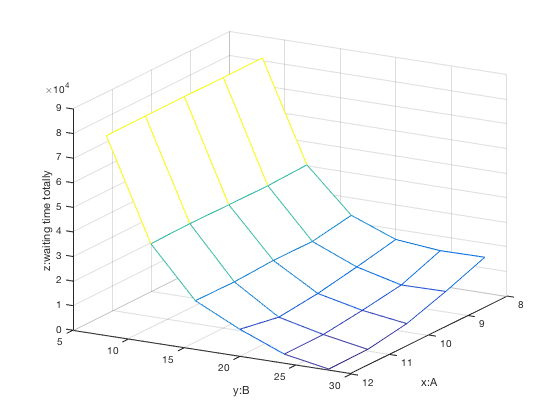
\includegraphics[width=6cm,height=6cm]{/Pic/waiting_total.png}
}
\subfigure[The standard deviation of the time spent on security checks] { \label{fig:waiting_total_std}
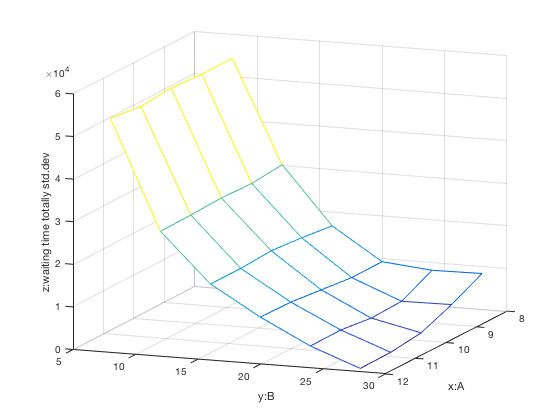
\includegraphics[width=6cm,height=6cm]{/Pic/waiting_tatally_stddev.png}
}
\subfigure[The average time passenger spent on screening with the pre-check passages] { \label{fig:pre_waiting_total}
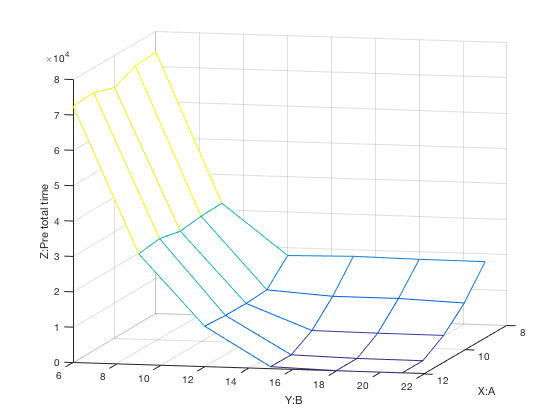
\includegraphics[width=6cm,height=6cm]{/Pic/pre_total_time.png}
}
\subfigure[The standard deviation of the time on screening with the pre-check passages] { \label{fig:pre_waiting_total_std}
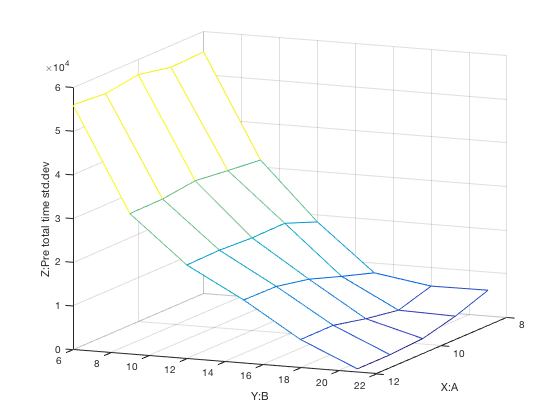
\includegraphics[width=6cm,height=6cm]{/Pic/pre_total_time_stddev.png}
}
\subfigure[The average time spent by all passenger] { \label{fig:pre_waiting_total_std}
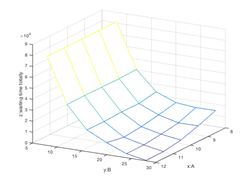
\includegraphics[width=6cm,height=6cm]{/Pic/7.png}
}
\subfigure[The standard deviation of the time spent by all passenger] { \label{fig:total_std}
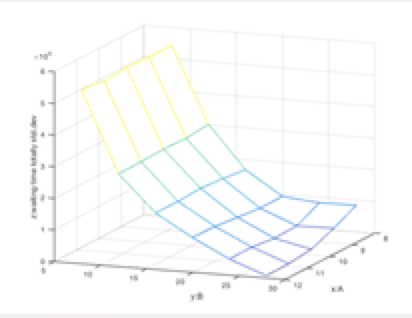
\includegraphics[width=6cm,height=6cm]{/Pic/8.png}
}
\caption{Figures}
\label{fig:Figures}
\end{figure}

According to the figure, with the increase in the number of workers in zone B, both the time-averaged and variance, there is a decreasing trend, that is, the improvement of queuing satisfaction. But when the number increased to a certain extent, the queuing satisfaction index will no longer be significantly improved, but tends to be stable, while the cost effect will still increase fast. Considering two factors, we take the number when the number of staff and equipment in zone A\&B increased to the average time spent and its variance began to change gently. As the optimized number of equipment staff ratio. That is, about 11 sets of equipment and staff in zone A checking identity information, and in zone B the equipment and staff checking belongings and body, for ordinary passengers, 18 sets, for the use of pre-inspection of passengers with 6 sets.( 3: 1 ratio of the information given from the title).

\subsection{Improve 3}
In addition to the above optimization transformation, we can also work on the internal security transformation process. Such as in the most congested zone B, We take into account that the majority of the time is spent on the inspection of the passengers by the staff, and the belongings is checked by the conveyor belt at a reliable speed. So we can on the basis of in each of the original conveyor belt is equipped with one staff checking body, add staff to the side of the belt to improve the efficiency of the zone B, and shorten the time. In order to reflect the optimization results, we may wish to assume that the number of B to add staff, to make the average time in the B zone inspection decreased by 20\%. After that we run the script again, the results are as followed:

\begin{figure}[H]
\centering
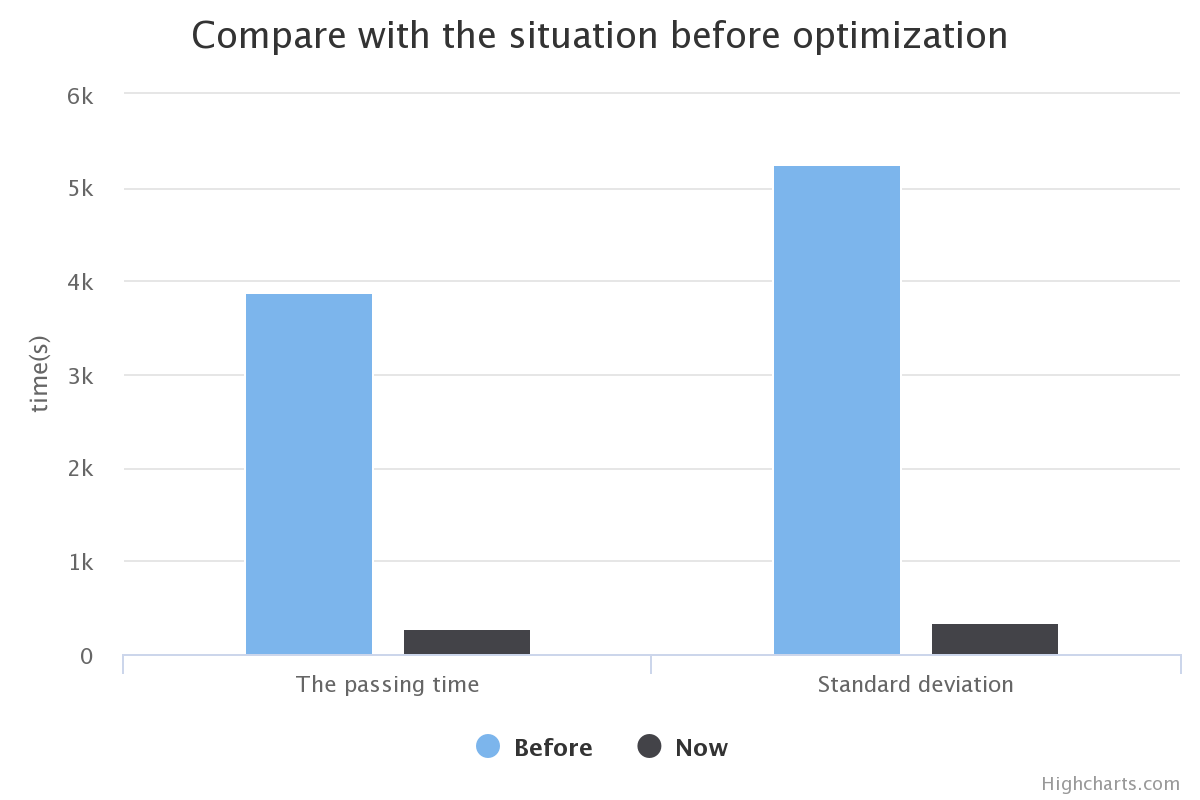
\includegraphics[width=14cm,height=8cm]{/Pic/缩短百分之二十的优化图.png}
\caption{Compare with the situation before optimization}\label{fig:Compare_Pic}
\end{figure}


According to the above figure, the appropriate number of staff to add in zone B can significantly improve work efficiency, reduce the time spent by passengers, improve passenger queuing satisfaction index.











%6 问题三模型建立与求解
%!TEX root = mcmpaper.tex
\section{problem c model design}
In order to study the impact of cultural differences on the airport security model, we analyzed the following two factors separately:
\subsection{Cultural differences}
\begin{enumerate}
	\item Travelers in some countries and regions are generally slow or fast, and their actions, including walking, baggage collection, taking documents, shoes off shoes, etc. The time cost will be longer or shorter than others . This will inevitably lead to the entire security process longer or shorter, the standard deviation will also be affected. Specifically, this cultural difference is quantified to the data is, the time required in zone A and B to check will be longer or shorter. In the following analysis, we assume that the average moving speed of the country is 10\% slower or faster than the rest.
	\item the passengers of some countries and regions have a free and independent character traits, they are common simple backpackers, travel with only one or two bags. While others are characterized by a conservative moderation character, they travel generally will bring a lot of belongings. This cultural difference in the airport security process is reflected in the zone B, they will spend less or more time compared to   passengers of other regions in the collection of belongings. In the following analysis, we assume that the average speed of the country is 10\% slower or faster in the zone B than the rest.
\end{enumerate}

Based on the above cultural differences, adjust the processing time of A and B regions, and re-simulate the corresponding data to carry out sensitivity analysis. The result is showed as followed:

\begin{table}[H]
\centering
\caption{The Influence of Cultural Difference on Time}\label{tab:cul_diff}
\begin{tabular}{|*{6}{r|}}
\hline
\multicolumn{2}{|c|}{\multirow{2}*{}}
& \multicolumn{2}{|c|}{Global Speed(1)} & \multicolumn{2}{|c|}{Zone B Speed(2)}\\\cline{3-6}
\multicolumn{2}{|c|}{}  & +10\%   & -10\% & +10\% & -10\%\\\hline
\multirow{1}*{Average time}
& \% & -72.4   & 30.9 & -51.5 & 25.3 \\\hline
\multirow{1}*{The variance of mean time}
& \% & -72.5   & 31.5 & -58.6 & 27.6 \\\hline
\end{tabular}
\end{table}

According to the table above, we can know what measures should be taken for each of the two different cultural. For the cultural differences 1, we need to properly adjust the number of equipment and staff of zone A\&B, to meet the changes in the speed of passenger movement. If the passenger is slower, you need to increase the number of equipment and staff of zone A\&B, if faster, take the contrary. For cultural differences 2, we need to properly adjust and the number of the equipment and staff of zone B to accommodate the number of passengers carrying belongings backpack. If passengers of a region carrying generally more bags backpack, it should be appropriate to increase the number of the equipment and staff of zone B, if less, take the contrary.


%7 合理化建议
%!TEX root = mcmpaper.tex
\section{Proposals}
Based on the above model as well as their analysis. In order to take full advantage of airport's security equipment and improve the efficiency of the staff and reduce the time of through the security zone and reduce the difference between each other. We would like to make the following recommendations to the safety management:
\begin{enumerate}
	\item Reasonable arrangements for flight time and the original peak hours of flights to be adjusted. Make the flight 24 hours a day evenly distributed. 
 	\item Make full use of equipment and staff in zone A. We can cancel the diversion in zone A, passengers who buy the pre-check service go to the pre-check channel in zone B.
 	\item Reasonably increase the number of equipment and staff in each zone. For example, for the study of the object O'Hare Airport, after our modeling and analysis we can see that zone A has 11 sets of equipment to identify passengers, zone B's regular channel has 18 sets of equipment to check baggage and passengers and pre-check channel has 6. Such a combination is more appropriate.
 	\item Reasonably increase the number of staff in the zone B to carry out physical examination of passengers to make full use of the conveyor belt efficiency and speed up the inspection speed of  zone B.
 	\item In the second improvement of question b, we find that passengers using pre-check channels don't spend less time than regular tourists. This may be related to the fact that more and more people in the USA are purchasing pre-check services and the probability of most of these people traveling by plane is very high. So the pre-check channel has not been fully utilized, when the passenger traffic is large, the airport can open serveral pre-check channel.
 	\item Airport security department needs to properly adjust the security procedures according to the differences between regions and regional culture. For example, people in some region may like to bring a lot of belongings, then it is appropriate to increase the zone B equipment and the number of staff and so on. Of course these improvements should be based on the specific regional culture and the specific situation. We need to try again and again to get the final program.
\end{enumerate}



%!TEX root = mcmpaper.tex
\section{Model Testing}
In order to further test the model we have established, we collected data from the Beijing Capital International Airport in China through actual investigation. According to the survey, 24 million people go into the Beijing International Airport every day. We put this data into our model. After simulation by computer, we come to the conclusion that the Beijing International Airport needs 72 sets of equipment and staff. In fact, the Beijing Capital International Airport has about 90 security entrance and it will open about 60-80 security entrance according the passengers traffic. This fact is very similar to our results and proves that the model we built is very reasonable and correct.

%8
%!TEX root = mcmpaper.tex
\section{Advantages and disadvantages and improvement}
\subsection{Advantages}
\begin{enumerate}
\item It is reasonable to assume that the hypothesis we set up before the model is based on the facts and the meaning of the study
\item The queuing theory we use to model the passenger's experience, which is difficult to measure directly, is represented by quantifiable indicators so that the passenger's experience can be compared with each other.
\item The data we get from simulation by computer has great scientific and reference value.
\item Through the image can be more obvious to see the appropriate solution.
\item The method we used can be applied to any airport.
\item The optimization recommendations we have given are practical and cost-effective, and are practical solutions.
\end{enumerate}

\subsection{Disadvantages}
\begin{enumerate}
\item The model established in this paper does not take into account the initial value of the number of queues in the simulation. We set the intial value 0. This will result in a certain impact. \textbf{The corresponding improvement scheme is to extend the period of simulation and get the steady state solution.}
\item The results obtained in this paper vary with the traffic volume, so the results can not be directly applied to other airports
\item We ignore the details of the security process for the impact of the results. For example, different staffs work differently and so on. \textbf{The corresponding improvement is that through a large zone of field investigation and data collection We can calculate the specific details of the results of our modeling and analysis of the specific impact of the quantified as a result of the variables into the model to improve the model.}
\end{enumerate}


%附录
%\input{Appendices}

\newpage

\clearpage
\phantomsection
\addcontentsline{toc}{section}{Reference} %向目录中添加条目,以章的名义
\bibliography{mybibtex}
\newpage
\addcontentsline{toc}{section}{Appendix} %向目录中添加条目,以章的名义
% !TEX root = mcmpaper.tex

\section*{Appendix}
\lstset{frame=tb,
  language=Java,
  aboveskip=3mm,
  belowskip=3mm,
  showstringspaces=false,
  columns=flexible,
  basicstyle={\small\ttfamily},
  numbers=none,
  numberstyle=\tiny\color{gray},
  keywordstyle=\color{blue},
  commentstyle=\color{dkgreen},
  stringstyle=\color{mauve},
  breaklines=true,
  breakatwhitespace=true
  tabsize=3
}

\definecolor{dkgreen}{rgb}{0,0.6,0}
\definecolor{gray}{rgb}{0.5,0.5,0.5}
\definecolor{mauve}{rgb}{0.58,0,0.82}


\subsection*{Emulation program core code}
\begin{lstlisting}
/**
 * Control time.
 */
public class TimeController {
    private Integer timeCounter;

    public TimeController(){
        timeCounter = 0;
    }

    public Integer getTimeCounter() {
        return timeCounter;
    }

    public void setTimeCounter(Integer timeCounter) {
        this.timeCounter = timeCounter;
    }

    public void tick(){
        timeCounter++;
    }
}

/**
 * Control Passenger
 */
public class PassengerController {
    private Integer passengerCounter;
    private Queue<Integer> dl;
    private FileWriter fileWriter;
    private ArrayList<Integer> timeRep;

    public PassengerController(FileWriter fileWriter){
        timeRep = new ArrayList<>();
        this.fileWriter = fileWriter;
        passengerCounter = 0;
        dl = new LinkedList<>();
        int count = 0;
        for (int i = 0; i < 75000; i++){
            count += Math.round(-1.152 * Math.log(Math.random()));
            dl.add(count);
        }
    }

    public Integer getPassengerCounter() {
        return passengerCounter;
    }

    public void setPassengerCounter(Integer passengerCounter) {
        this.passengerCounter = passengerCounter;
    }

    public ArrayList<Passenger> getPassenger(Integer time){
        ArrayList<Passenger> passengers = new ArrayList<>();
        while (!dl.isEmpty() && time.compareTo(dl.peek()) == 0){
            dl.poll();
            Passenger passenger;
            if (Math.random() * 100 <= 45){
                passenger = new Passenger(passengerCounter, time, 0, 0, true, fileWriter);
            }else{
                passenger = new Passenger(passengerCounter, time, 0, 0, false, fileWriter);
            }
            passengerCounter++;
            passengers.add(passenger);
        }

        return passengers;
    }

    public Integer getTime(){
        return 1;
    }
}

/**
 * Main method
 */
public static void main(String [] args) throws IOException {
        System.out.println("Airport simulation");

        init();

        while(timeController.getTimeCounter() < 3600 * 24 * 4){
            ArrayList<Passenger> passengers = passengerController.getPassenger(timeController.getTimeCounter());
            if(passengers.size() != 0){
                for (Passenger passenger : passengers){
                    passenger.setStartA(timeController.getTimeCounter());
                    pointA.add(passenger);
                }
            }
            if (timeController.getTimeCounter() % 60 == 0){
                pointA.action(true, timeController.getTimeCounter());
                bArea.action(true, timeController.getTimeCounter());
                cArea.action(true, timeController.getTimeCounter());
                pointD.action(true, timeController.getTimeCounter());
            }else{
                pointA.action(false, timeController.getTimeCounter());
                bArea.action(false, timeController.getTimeCounter());
                cArea.action(false, timeController.getTimeCounter());
                pointD.action(false, timeController.getTimeCounter());
            }

            timeController.tick();
        }
        exit();
    }
}

/**
 * Passenger.
 */
public class Passenger {
    private Integer id;
    private Integer arriveTime;
    private Integer exitTime;
    private Integer state;
    private Boolean isPre;
    private Integer doing;
    private FileWriter fileWriter;
    private Integer startA;
    private Integer endA;
    private Integer startB;
    private Integer endB;
    private Integer startC;
    private Integer endC;
    private Integer startD;
    private Integer endD;


    public Passenger(Integer id, Integer arriveTime, Integer state, Integer doing, Boolean isPre, FileWriter fileWriter){
        this.id = id;
        this.arriveTime = arriveTime;
        this.state = state;
        this.doing = doing;
        this.fileWriter = fileWriter;
        this.isPre = isPre;

        startA = 0;
        endA = 0;
        startB = 0;
        endB = 0;
        startC = 0;
        endC = 0;
        startD = 0;
        endD = 0;
    }

    /* method */
    public void writing() throws IOException {
        fileWriter.write(id + " " + arriveTime + " " + exitTime + " " + String.valueOf(endA - startA) + " " +
                String.valueOf(endB - startB) + " " + String.valueOf(endC - startC) + " " +
                String.valueOf(endD - startD) + " " + String.valueOf(getPre()) + "\n");
        fileWriter.flush();
    }
}

/**
 * A Area
 */
public class PointA extends Point {
    private FileWriter fileWriterWaiting;
    private FileWriter fileWriterPassing;
    private BArea next;
    private ArrayList<Passenger> dealPassengers;
    private Integer countPassenger;

    public PointA(Integer name, BArea pointBPre, FileWriter fileWriterWaiting, FileWriter fileWriterPassing) {
        super(name);
        next = pointBPre;
        countPassenger = 0;
        this.fileWriterPassing = fileWriterPassing;
        this.fileWriterWaiting = fileWriterWaiting;
        dealPassengers = new ArrayList<>();
    }

    @Override
    public void action(Boolean flag, Integer time){

        while(getWaitingList().size() != 0 && dealPassengers.size() < 12){
            Passenger passenger = getWaitingList().poll();

            passenger.setDoing(((int) ( (Math.round(Math.random() * 8) + 7))));
            dealPassengers.add(passenger);
        }


        ArrayList<Passenger> temp = new ArrayList<>();

        for (Passenger passenger : dealPassengers){
            temp.add(passenger);
        }

        for (Passenger passenger : temp){
            deal(passenger, time);
        }

        // record
        try {
            fileWriterWaiting.write(String.valueOf(getWaitingList().size()) + "\n");
            fileWriterWaiting.flush();
            if (flag){
                fileWriterPassing.write(String.valueOf(countPassenger) + "\n");
                fileWriterPassing.flush();
                countPassenger = 0;
            }
        } catch (IOException e) {
            e.printStackTrace();
        }

    }

    public void deal(Passenger passenger, Integer time){
        if (passenger != null){
            if (passenger.getDoing() > 0){
                passenger.setDoing(passenger.getDoing() - 1);
            }else{
                countPassenger++;
                passenger.setEndA(time);
                passenger.setStartB(time);
                if (passenger.getPre()){
                    // Pre
                    next.getBsPre().get(gotoB(7)).add(passenger);
                }else{
                    // regular
                    next.getBs().get(gotoB(21)).add(passenger);
                }
                for (int i = 0; i < dealPassengers.size(); i++){
                    if (dealPassengers.get(i).equals(passenger)){
                        dealPassengers.remove(i);
                        break;
                    }
                }
            }
        }
    }

    public Integer gotoB(int n){
        Integer num = (int) (Math.random() * n);
        return num;
    }
}

/**
 * B Area
 */
public class PointB extends Point {
    private FileWriter fileWriterWaiting;
    private FileWriter fileWriterPassing;
    private Passenger passenger;
    private CArea next1;
    private PointD next2;
    private Integer countPassenger;

    public PointB(Integer name, CArea cArea, PointD pointD) throws IOException {
        super(name);

        next1 = cArea;
        next2 = pointD;
        countPassenger = 0;

        fileWriterWaiting = new FileWriter(String.valueOf(name) + "_B_Waiting.txt");
        fileWriterWaiting.write("B " + String.valueOf(name) + " Waiting Record\n");
        fileWriterWaiting.flush();

        fileWriterPassing = new FileWriter(String.valueOf(name) + "_B_Passing.txt");
        fileWriterPassing.write("B " + String.valueOf(name) + " Passing Record\n");
        fileWriterPassing.flush();
    }

    @Override
    public void action(Boolean flag, Integer time){
        if (passenger == null && getWaitingList().size() != 0){
            passenger = getWaitingList().poll();

            passenger.setDoing(getTime());
        }

        if (passenger != null){
            if (passenger.getDoing() > 0){
                passenger.setDoing(passenger.getDoing() - 1);
            }else{
                countPassenger++;
                passenger.setEndB(time);
                if (Math.random() * 100 < 2){
                    // to d
                    passenger.setStartD(time);
                    next2.add(passenger);
                }else {
                    // to c
                    passenger.setStartC(time);
                    if (!passenger.getPre()) {
                        next1.getCs().get(gotoC(21)).add(passenger);
                    }else{
                        next1.getCbs().get(gotoC(7)).add(passenger);
                    }
                }
                passenger = null;
            }
        }

        // record
        try {
            fileWriterWaiting.write(String.valueOf(getWaitingList().size()) + "\n");
            fileWriterWaiting.flush();
            if (flag){
                fileWriterPassing.write(String.valueOf(countPassenger) + "\n");
                fileWriterPassing.flush();
                countPassenger = 0;
            }
        } catch (IOException e) {
            e.printStackTrace();
        }
    }

    public void exit() throws IOException {
        fileWriterPassing.close();
        fileWriterWaiting.close();
    }

    public Integer getTime(){
        Integer num1 = (int) Math.round(Math.random() * 5 + 24);
        Integer num2 = (int) Math.round(Math.random() * 5 + 44);

        if (Math.random() > 0.1){
            return num1;
        }else {
            return num2;
        }
    }

    public Integer gotoC(int n){
        Integer num = (int) (Math.random() * n);
        return num;
    }
}

/**
 * C Area
 */
public class PointC extends Point {
    private FileWriter fileWriterWaiting;
    private FileWriter fileWriterPassing;
    private Passenger passenger;
    private Integer countPassenger;
    public PointC(Integer name) throws IOException {
        super(name);

        fileWriterWaiting = new FileWriter(String.valueOf(name) + "_C_Waiting.txt");
        fileWriterWaiting.write("C " + String.valueOf(name) + " Waiting Record\n");
        fileWriterWaiting.flush();

        fileWriterPassing = new FileWriter(String.valueOf(name) + "_C_Passing.txt");
        fileWriterPassing.write("C " + String.valueOf(name) + " Passing Record\n");
        fileWriterPassing.flush();
    }

    @Override
    public void action(Boolean flag, Integer time) throws IOException {
        if (passenger == null && getWaitingList().size() != 0){
            passenger = getWaitingList().poll();
            passenger.setDoing((int) Math.round(Math.random() * 5 + 4));
        }

        if (passenger != null){
            if (passenger.getDoing() > 0){
                passenger.setDoing(passenger.getDoing() - 1);
            }else{
                countPassenger++;
                passenger.setEndC(time);
                passenger.setExitTime(time);
                passenger.writing();
                passenger = null;
            }
        }

        // record
        try {
            fileWriterWaiting.write(String.valueOf(getWaitingList().size()) + "\n");
            fileWriterWaiting.flush();
            if (flag){
                fileWriterPassing.write(String.valueOf(countPassenger) + "\n");
                fileWriterPassing.flush();
                countPassenger = 0;
            }
        } catch (IOException e) {
            e.printStackTrace();
        }
    }

    public void exit() throws IOException {
        fileWriterPassing.close();
        fileWriterWaiting.close();
    }
}

/**
 * D Area
 */
public class PointD extends Point {
    private FileWriter fileWriterWaiting;
    private FileWriter fileWriterPassing;
    private ArrayList<Passenger> dealPassengers;
    private Integer countPassenger;
    public PointD(Integer name, FileWriter fileWriterWaiting, FileWriter fileWriterPassing) {
        super(name);
        this.fileWriterPassing = fileWriterPassing;
        this.fileWriterWaiting = fileWriterWaiting;
        dealPassengers = new ArrayList<>();
        countPassenger = 0;
    }

    @Override
    public void action(Boolean flag, Integer time) throws IOException {
        while(getWaitingList().size() != 0 && dealPassengers.size() < 4){
            Passenger passenger = getWaitingList().poll();
            passenger.setDoing(60);
            dealPassengers.add(passenger);
        }

        ArrayList<Passenger> temp = new ArrayList<>();

        for (Passenger passenger : dealPassengers){
            temp.add(passenger);
        }

        for (Passenger passenger : temp){
            deal(passenger, time);
        }

        // record
        try {
            fileWriterWaiting.write(String.valueOf(getWaitingList().size()) + "\n");
            fileWriterWaiting.flush();
            if (flag){
                fileWriterPassing.write(String.valueOf(countPassenger) + "\n");
                fileWriterPassing.flush();
                countPassenger = 0;
            }
        } catch (IOException e) {
            e.printStackTrace();
        }

    }

    public void deal(Passenger passenger, Integer time) throws IOException {
        if (passenger != null){
            if (passenger.getDoing() > 0){
                passenger.setDoing(passenger.getDoing() - 1);
            }else{
                countPassenger++;
                passenger.setEndD(time);
                passenger.setExitTime(time);
                passenger.writing();
                for (int i = 0; i < dealPassengers.size(); i++){
                    if (dealPassengers.get(i).equals(passenger)){
                        dealPassengers.remove(i);
                        break;
                    }
                }
            }
        }
    }
}

\end{lstlisting}



\end{document}
% ----- End of Document Body -----
























% %=====================导=======言==============================
% % \documentclass[a4paper,12pt]{article}
% \documentclass[a4paper,12pt,titlepage]{article}
% %======================Include Packages========================

% \usepackage[14526]{MCMthesis}  %队号在这里填写
% % \problem{C}
% %===============设置正文和数学字体=============================
% %字体定义,大家可以参看网站:http://www.tug.dk/FontCatalogue/
% %有100多字体,可以复制放在这里设置字体,一般用默认字体即可。
% %有些字体需要安装一些字体文件,注意辨别。
% %我参照 MCM论文集的字体 使用如下宏包来定制字体。
% \usepackage{palatino}

% %设置段落之间的距离,若不需要删除或者注释掉即可。
% \setlength\parskip{.8\baselineskip}

% %各种宏包
% \usepackage{caption}
% \usepackage{graphicx}
% \usepackage{array}

% %%%%%%%%%%%%%%%%%%%%%%%%%%%%%%%%%%%%%%%%%%%%%%%%%%%%%%%%%%%%%%%%%%%
% %%%%%%%%%%%%%%%%%%$$$$$$$==正文开始==$$$$$$$%%%%%%%%%%%%%%%%%%%%%%%
% %%%%%%%%%%%%%%%%%%%%%%%%%%%%%%%%%%%%%%%%%%%%%%%%%%%%%%%%%%%%%%%%%%%

% %==========================论文标题===============================
% % \title{The \LaTeX Template for  MCM Version4.0}
% % \author{\small Edit by:China\TeX{} \url{http://blog.sina.com.cn/wangzhaoli11}}
% % \date{\today}
% %=================================================================
% %==================================================================
% \begin{document}
% % \maketitle
% %\thispagestyle{empty}
% %==================================================================

% %\vspace*{\fill}
% %====================摘=======要===================================
% %!TEX root = mcmpaper.tex
\begin{abstract}
In order to protect people's security and to provide more convenience, the reasonable setting of the airport security procedures is of great importance. This paper take the airport security inspection process as the main research object and use relevant theory, through the establishment and analysis of the model to find the bottlenecks in the current security inspection process and optimize the security system to get the best solution. And this paper also consider the influence of cultural differences and give some reasonable suggestions.\\
To establish the initial model, this paper first analyze the information given by the subject, and make reasonable assumptions. This paper use the queuing theory model to describe the queueing situation. And we transform the real airport security inspection system to a Petri net to simplify calculation. Then this paper use programming method to simulate the flow of passengers between various zones through computer simulation and give out the average passing time and its standard deviation on the chart, it's obvious that Zone A and B are the bottlenecks in the security process.\\
To optimizing the bottlenecks, this paper establish a evaluation index system including queuing satisfaction and cost effect. Firstly, we can increase the personnel and equipment in Zone A and B, but the values can not increase without limit considering the cost of modifications. Therefore, by this system, we can find out values that can not only greatly optimize the wait time but also save money. The result show that 11 officers in Zone A and 24 sets of equipment in Zone B will be the best program which can save over 50\% time. Besides, we can adjust the procedures, for the most crowded and time consuming Zone B, we can moderately increase the officer to sharply reduce the congestion of passengers and improve the travel experience.
\\
In order to find out the effect of different cultures, two culture differences are mentioned as analysis object. This paper quantified the influence and then change the corresponding parameter in the simulation program to get the result to make sensitivity analysis. And proposes are also given to accommodate these differences. For example, more equipment should be offered in places with more belongings.

\end{abstract}
                                              %
% \newpage                                                          %
% %==================================================================


% %====================生=成=目=录===================================
% \tableofcontents                                                  %                                            %
% \newpage                                                          %
% %==================================================================
% %!TEX root = mcmpaper.tex

\newcommand\degree{^{\circ}}

%1 问题重述
%!TEX root = mcmpaper.tex

%======================问题重述====================================
\section{Problems restatement}

\subsection{Introduction}
Following the terrorist attacks in the US on September 11,2001, airport security has been significantly enhanced throughout the world, the security situation has also been improved. In order to ensure the safety of all passengers, every passenger must pass the security checkpoint before entering the airport, but a lot of inconvenience is also caused. How to maximize security while minimizing inconvenience to passengers, the research of this problem is of great significance in the present air traffic business.

\subsection{Restatement}
The flow of US airport security checkpoints is known as followed: First line up to check the identification and board documents in Zone A, then check the body and belongings in Zone B, then collect belongings in Zone C, if there's nothing wrong, then you can leave. Passengers that fail this step receive a pat-down inspection in Zone D.
Besides, approximately 45\% of passengers enroll in a program called Pre-Check for trusted travelers, these passengers pay 85\$ to receive a background check and enjoy a separate screening process for five years, in this way they can save some time in Zone B. Data of time in each step has been offered.
\par
Our tasks are:
\begin{enumerate}
  \item Establish a reasonable model to identify bottlenecks.
  \item Develop two or more potential modifications to the current process to improve passenger throughput and reduce variance in wait time.
  \item Consider cultural differences and analyze how can the security system accommodate these differences.
  \item Propose policy and procedural recommendations for the security managers based on the model.
\end{enumerate}


%2 问题分析
%!TEX root = mcmpaper.tex
\section{Model Analysis}
\subsection{Analysis of problem a}
% 第一问分析
As we are aware of the detailed process of security check and data of each step, we can get the time every passenger spent in each Zone of the security checkpoint. After making reasonable assumption, we can simulate out the average wait time and variance in wait time of passengers in the security checkpoint by computer programming. To establish the Model 1 and identify the bottlenecks and problematic Zones.
\subsection{Analysis of problem b}
% 第二问分析
Based on the Model 1, we should develop modifications to improve passenger throughput and reduce variance in wait time. Firstly we set the Zone A for both Pre-check and regular check to use, then we adjust the number of officers in Zone A and Pre-check and regular lanes in Zone B. Because the bottleneck has been identified in Model 1, through traversal adjustment to the number of lanes in a certain range, we can get the passenger throughput and wait time variance in each condition. Considering the cost, we should choose the best number of Zone A officer and lanes in Zone B. In addition, the details of the process can also be changed such as adding another security officer next to the belt in Zone B to slow down the blockage of manual check.

\subsection{Analysis of problem c}
% 第三问分析
In this problem we consider how cultural differences may impact the way in which passenger's process through checkpoints as a sensitivity analysis. We take two cultural differences into consideration. One is passengers in some places are much slower, which will result in a longer time of the whole process. The other is that in some area like Italy people enjoy chic lifestyle and wouldn't like to take much belongings, so the time in Zone B will reduce. We take these two differences into simulation separately and make sensitivity analysis.


%3 模型假设
%!TEX root = mcmpaper.tex

%======================Model Assumptions====================================
\section{Model Assumptions}
The model should be based on the six following assumptions:
\begin{itemize}
  \item Assumption 1:The passengers are slower than belongings: This is based on our life experience.
  \item Assumption 2:Develop two or more potential modifications to the current process to improve passenger throughput and reduce variance in wait time.
  \item Assumption 3:The number of passengers to the airport is 75000: We take Chicago O'Hare Airport as an example, and we find the passenger traffic in the related news.
  \item Assumption 4:The time required for the officer to perform security checks is normally distributed.
  \item Assumption 5:There is not any emergency event happened in airport.
  \item Assumption 6:Passengers with Pre-check qualification are all queued at the Pre-check lanes.
\end{itemize}


%4 符号申明
%!TEX root = mcmpaper.tex

%==================================符号声明========================================
\section{Notations}
\begin{table}[H]
\centering
\caption{Notations}\label{tab:notations}
\begin{tabular}{|c|c|c|}
\hline
Notations& Definition& Dimension\\ \hline
$P_{i}$& The probability of an event & None \\
\hline
$T_{i}$& The elapsed time of an event & s \\\hline
P & Queuing satisfaction & None \\\hline
L & The time required to pass all security checks & s \\\hline
S & The standard deviation of the security period & s \\\hline
C & Cost effect & None \\\hline
$A_{0}$ & The initial state of the equipment personnel in Zone A & set \\\hline
$A_{t}$ & Improved zone A equipment personnel & set \\\hline
$B_{0}$ & The initial state of the equipment personnel in Zone B & set \\\hline
$B_{t}$ & Improved zone B equipment personnel & set \\
\hline
\end{tabular}
\end{table}

%4 问题一模型建立与求解
%!TEX root = mcmpaper.tex

%===============================模型设计============================================
\section{Problem a model design}
\subsection{The distribution of tourists}
The distribution of passengers into the airport is as followed:
\par
According to the assumption 2, passengers arrive at Poisson flow. The probability of the total number of passengers arriving at the airport in time t is as followed:

% \begin{equation}
% \left.
% \begin{aligned}[b]
%   f(x)=\frac{1}{\sqrt{2\pi }*3.7926}*e^{-\frac{(x-11.2125)^2}{2*14.384}}
% \end{aligned}
% \right.
% \end{equation}

\begin{equation}
\left.
\begin{aligned}[b]
	{P_{n}}(t)=\frac{(\lambda t)^{n}}{n!}*e^{-\lambda t}
\end{aligned}
\right.
\end{equation}

parameter $\lambda$ is the average number of the passengers arrive at unit time. According to 24 hours a day, the total passenger flow is 75000, we calculate out $\lambda$=0.8681 p/s.

\begin{equation}
\left.
\begin{aligned}[b]
	{P_{n}}(t)=\frac{(0.8681t)^{n}}{n!}*e^{-0.8681t}
\end{aligned}
\right.
\end{equation}

the time interval between any two passengers meet the negative exponential distribution $\lambda$=0.8681 p/s, the Distribution function:

\begin{equation}
\left.
\begin{aligned}[b]
	F(t)=1-e^{-0.8681t}~ ~t\geq 0
\end{aligned}
\right.
\end{equation}

Set $R=F(t)$, therefore R is evenly distributed in (0,1). Through inverse transformation we get:

\begin{equation}
\left.
\begin{aligned}
	T=-\frac{1}{0.8681}ln(1-R)=-1.1519ln(1-R)
\end{aligned}
\right.
\end{equation}

Set $U=1-R$,and $U$ is also evenly distributed in $(0,1)$. The time interval $T$ between any two passengers is a random number subject to exponential distribution:

\begin{equation}
\left.
\begin{aligned}
	T=-1.1519ln U
\end{aligned}
\right.
\end{equation}

\subsection{The security process}
According to the assumptions and data offered in the Excel, we can draw a airport security Petri Net Model as followed:

\subsubsection*{Petri Net}
Petri Net is an effective model tool to describe and analyze the system with concurrent and synchronous features. We consider the security check as a system, which is synchronized and concurrent. Using time parameter based on the actual situation to analyze the time of model. Then choose the Generalized Stochastic Petri Net, GSPN to modeling the security check process.

\begin{figure}[H]
\centering
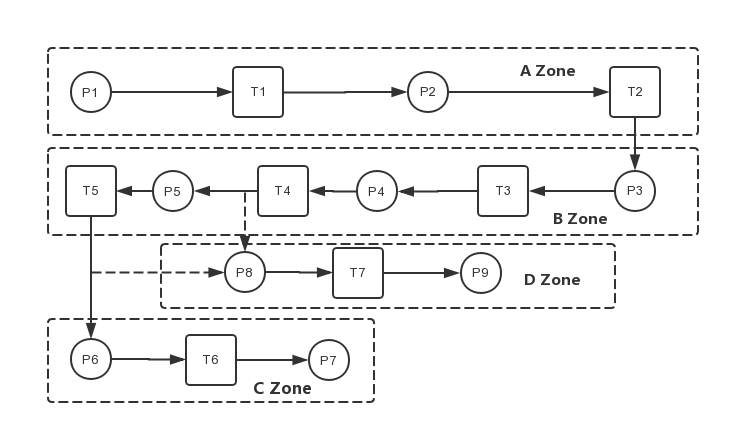
\includegraphics[width=17cm,height=12cm]{/Pic/patrymodel.png}
\caption{Petri network diagram}\label{fig:Petri_Pic}
\end{figure}



\subsubsection*{Symbols in the picture}
\begin{table}[H]
\centering
\caption{Notations}\label{tab:notations}
\begin{tabular}{|c|c|}
\hline
Symbol& Meaning\\
$P_{1}$& Arrivals at the airport \\
\hline
$P_{2}$& Passengers to start receiving identity checks \\\hline
$P_{3}$& Passengers waiting in the queue in Zone B to put their belongings to screening \\\hline
$P_{4}$& Passengers starting to put their belongings on the belt\\\hline
$P_{5}$& Passengers starting to go through scanner\\\hline
$P_{6}$& Passengers packing belongings in Zone C\\\hline
$P_{7}$& Passengers finished the whole process\\\hline
$P_{8}$& Passengers failed step receive a pat-down inspection\\\hline
$P_{9}$& Passengers finished the inspection in Zone D(10\%)
\\\hline
$T_{1}$& Time of waiting for identity verification \\\hline
$T_{2}$& Time of receiving the identity verification(average 11.21s, standard deviation 3.79s) \\\hline
$T_{3}$& Time of waiting for belongings screening\\\hline
$T_{4}$& Time of putting the belongings on the belt\\\hline
$T_{5}$& Time of receiving body inspection(average 41s, standard deviation 6.9s)\\\hline
$T_{6}$& Time of passengers to pack belongings
\\\hline
$T_{7}$& Time of receiving inspection in Zone D
\\\hline

\hline
\end{tabular}
\end{table}


\subsection{Model establishment and solution}
 Based on the above information we can carry out simulation of the airport flow by computer, here are the programming method:
\par
 The entities in the simulation program are composed of passengers, zone A, zone B, zone B and zone D, the controller consists of a time controller and a passenger controller. Here are the description of the relevant attributes and logical description:
\subsubsection*{Attributes Description:}
\paragraph*{Passenger:}
\begin{enumerate}
	\item Time to reach the airport
 	\item Time to leave the security zone
 	\item Whether to buy the  background check
 	\item Time to reach the zone A
 	\item Time to leave the zone A
  	\item Time to reach the zone B
 	\item Time to leave the zone B
 	\item Time to reach the zone C
 	\item Time to leave the zone C
 	\item Time to reach the zone D
 	\item Time to leave the zone D
\end{enumerate}
\paragraph*{Zone}
\begin{enumerate}
	\item Name
	\item The waiting list
\end{enumerate}

\subsubsection*{Logical Description:}
\begin{enumerate}
	\item The time controller increase the time by one second and ask the passenger controller how many passengers reaching the airport at that second. Then the passenger controller put the coming passengers into zone A's waiting list.
	\item The time controller informs all zones to take action
	\item Zone A Reduces the processing time by one for all passengers who are checking documents, then put the passengers who complete the task without problem into zone B's waiting list. Finally, take passengers from zone A's waiting list and set their processing time.
	\item Zone B Reduces the processing time by one for all passengers who are accepting checking, then put the passengers who complete the task without problem into zone C's waiting list and put the other problematic passengers into zone D's waiting list. Finally, take passengers from zone B's waiting list and set their processing time.
	\item Zone C Reduces the processing time by one for all passengers who are packing belongings, then record the data of passengers who complete the task.Finally, delete the passengers and take passengers from zone C's waiting list and set their processing time.
	\item Zone D Reduces the processing time by one for all passengers who are accepting addtional search, then record the data of passengers who complete the task.Finally, delete the passengers and take passengers from zone D's waiting list and set their processing time.
	\item Repeat step 1,2,3,4,5 until all passengers are deleted
	\item Run the script to extract the data and analysis
\end{enumerate}


\subsubsection*{Activity Diagram:}
\begin{figure}[H]
\centering
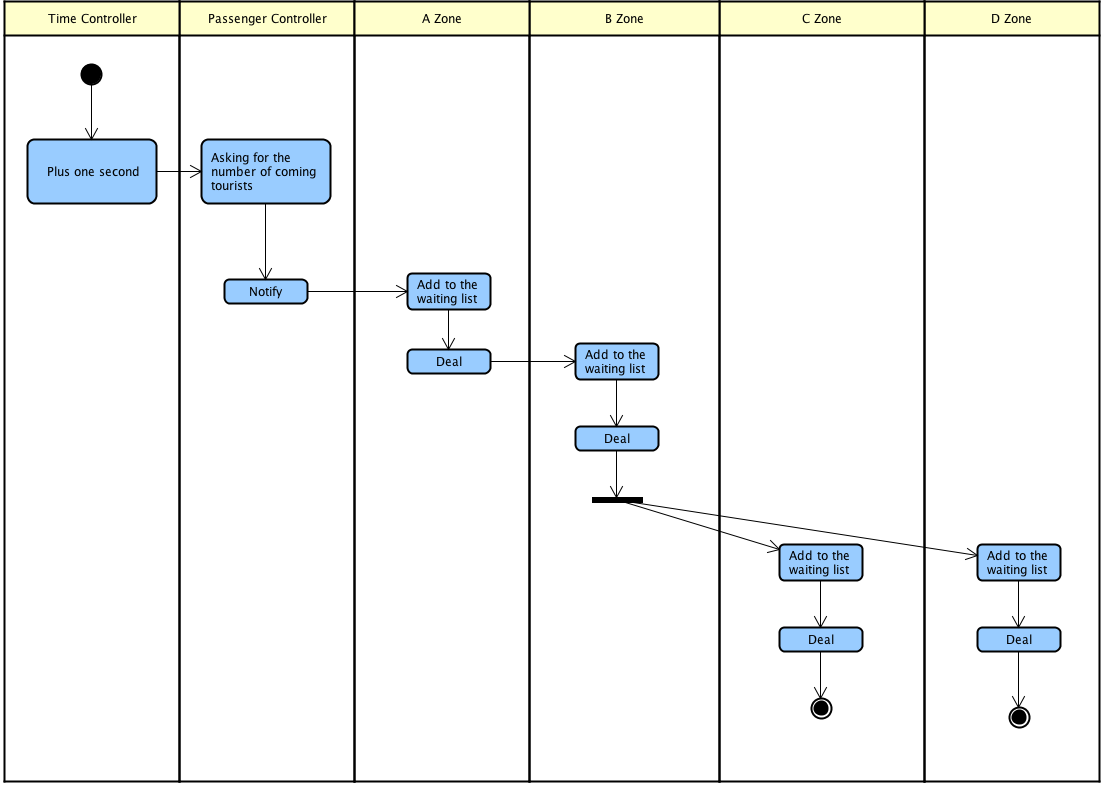
\includegraphics[width=14cm,height=8cm]{/Pic/activity_diagram.png}
\caption{Activity diagram}\label{fig:acd}
\end{figure}

\subsection{Model summary}
According to the above programming ideas for programming simulation, the average time of passengers waiting in each Zone is as followed:

\begin{figure}[H]
\centering
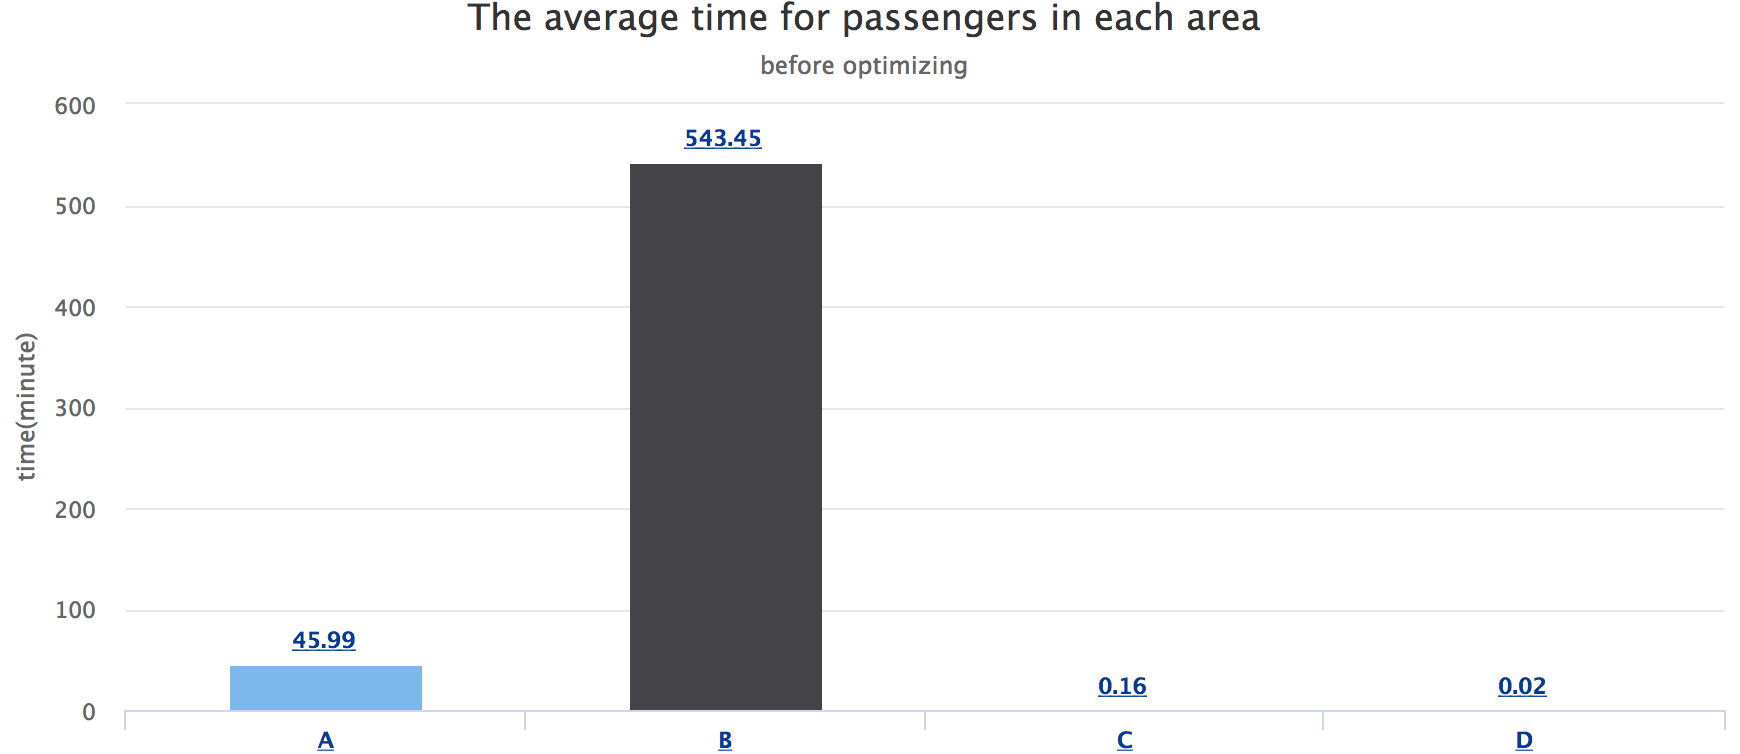
\includegraphics[width=14cm,height=8cm]{/Pic/第一问瓶颈图.png}
\caption{Bottleneck in process}\label{fig:bottleneck}
\end{figure}

We can conclude from the picture that \textbf{the time passengers spent in A and B are the most, which is hundreds times of C and D. So the bottlenecks are Zone A and B, which should be focusing optimized in our future modeling.}










%5 问题二模型建立与求解
%!TEX root = mcmpaper.tex
\section{problem b model design}
premise: In order to better measure our optimization effect, we introduce two parameters: queuing satisfaction, and cost effect.As explained below:

\begin{equation}
\left.
\begin{aligned}[b]
  P = \frac{1}{L*S}\footnotemark[1]
\end{aligned}
\right.
\end{equation}

\begin{equation}
\left.
\begin{aligned}[b]
  C=\frac{A_{t}}{A_{0}}+\frac{B_{t}}{B_{0}}
  \footnotemark[2]
\end{aligned}
\right.
\end{equation}

\footnotetext[1]{
	\textbf{P}: Queuing satisfaction\\ 
	\textbf{L}: The time required to pass all security checks;\\ 
	\textbf{S}: The standard deviation of the security period;
}

\footnotetext[2]{
	\textbf{$A_{0}$}: The initial state of the equipment personnel in zone A;\\ 
	\textbf{$A_{t}$}: Improved zone A's equipment personnel;\\ 
	\textbf{$B_{0}$}: The initial state of the equipment personnel in zone B;\\
	\textbf{$B_{t}$}: TImproved zone B's equipment personnel;
}

\subsection{Improve 1}
On the basis of Problem 1, we have recognized the bottleneck. In order to further improve the airport security throughput and reduce the waiting time difference, we first thought is to improve the security process of the zone A . As shown in the title, passengers waiting in zone A for identity verification are inspected at two locations, the travelers using the Pre-Check process and regular travelers. But for the process of identity verification, the use of Pre-Check process or not is not affected. So in order to make full use of each verification entrance of zone A, we cancel the respective queuing of passengers in zone A, and change to uniform distribution queuing.

\subsection{Improve 2}
Secondly, we need to adjust the number of security lanes ratio of every security zone. By the traversal adjustment of regional security lanes in a certain range of the number, we can get the time and its variance spent by travelers in each case. Considering the cost, from which to choose the best ratio.
\par
For this reason, we have made the following improvements to the program of Model 1:
Zone A, B, and C in the simulation program have a processing queue that can be resized. In this question, in order to simulate the number of different inspection lanes, we continue to adjust the parameters for ergodic solution, while running the script than the data obtained, and finally get the best combination.
\par
The result is as followed (Where X-axis represents the number of staff and equipment in zone A, and Y-axis represents the number of staff and equipment in zone B equipment.)

\begin{figure}[H]
\centering
\subfigure[The average time normal passenger spent on security checks] { \label{fig:Waiting_Total}
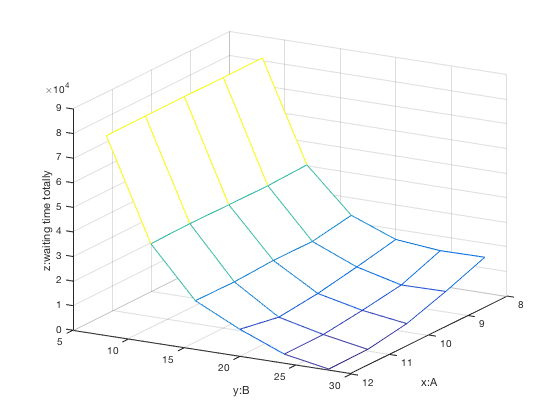
\includegraphics[width=6cm,height=6cm]{/Pic/waiting_total.png}
}
\subfigure[The standard deviation of the time spent on security checks] { \label{fig:waiting_total_std}
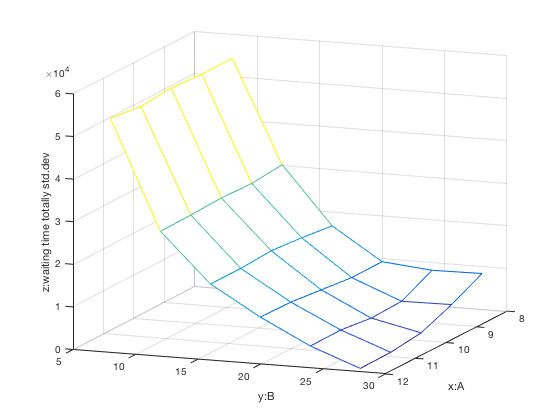
\includegraphics[width=6cm,height=6cm]{/Pic/waiting_tatally_stddev.png}
}
\subfigure[The average time passenger spent on screening with the pre-check passages] { \label{fig:pre_waiting_total}
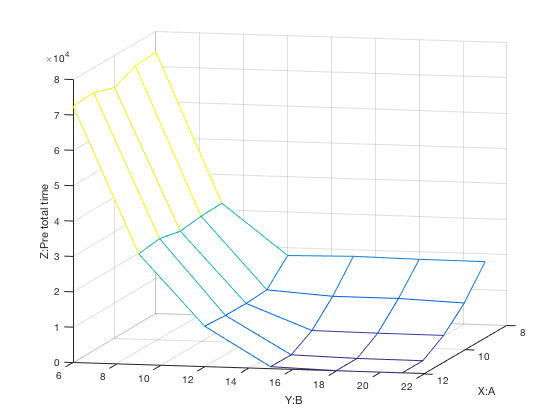
\includegraphics[width=6cm,height=6cm]{/Pic/pre_total_time.png}
}
\subfigure[The standard deviation of the time on screening with the pre-check passages] { \label{fig:pre_waiting_total_std}
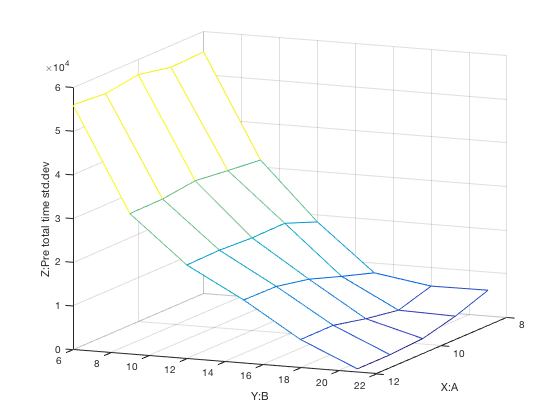
\includegraphics[width=6cm,height=6cm]{/Pic/pre_total_time_stddev.png}
}
\subfigure[The average time spent by all passenger] { \label{fig:pre_waiting_total_std}
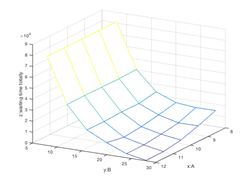
\includegraphics[width=6cm,height=6cm]{/Pic/7.png}
}
\subfigure[The standard deviation of the time spent by all passenger] { \label{fig:total_std}
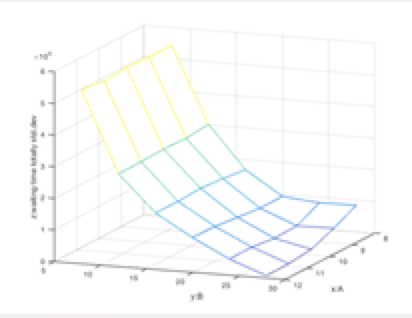
\includegraphics[width=6cm,height=6cm]{/Pic/8.png}
}
\caption{Figures}
\label{fig:Figures}
\end{figure}

According to the figure, with the increase in the number of workers in zone B, both the time-averaged and variance, there is a decreasing trend, that is, the improvement of queuing satisfaction. But when the number increased to a certain extent, the queuing satisfaction index will no longer be significantly improved, but tends to be stable, while the cost effect will still increase fast. Considering two factors, we take the number when the number of staff and equipment in zone A\&B increased to the average time spent and its variance began to change gently. As the optimized number of equipment staff ratio. That is, about 11 sets of equipment and staff in zone A checking identity information, and in zone B the equipment and staff checking belongings and body, for ordinary passengers, 18 sets, for the use of pre-inspection of passengers with 6 sets.( 3: 1 ratio of the information given from the title).

\subsection{Improve 3}
In addition to the above optimization transformation, we can also work on the internal security transformation process. Such as in the most congested zone B, We take into account that the majority of the time is spent on the inspection of the passengers by the staff, and the belongings is checked by the conveyor belt at a reliable speed. So we can on the basis of in each of the original conveyor belt is equipped with one staff checking body, add staff to the side of the belt to improve the efficiency of the zone B, and shorten the time. In order to reflect the optimization results, we may wish to assume that the number of B to add staff, to make the average time in the B zone inspection decreased by 20\%. After that we run the script again, the results are as followed:

\begin{figure}[H]
\centering
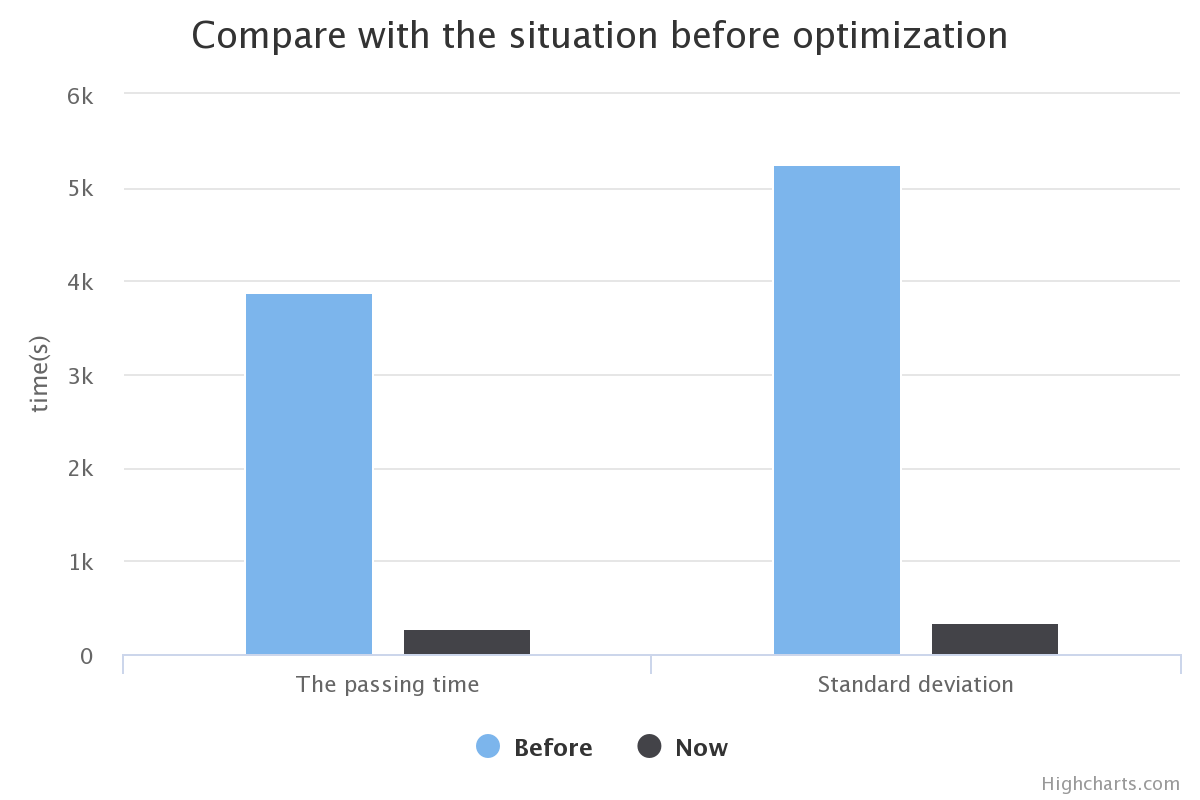
\includegraphics[width=14cm,height=8cm]{/Pic/缩短百分之二十的优化图.png}
\caption{Compare with the situation before optimization}\label{fig:Compare_Pic}
\end{figure}


According to the above figure, the appropriate number of staff to add in zone B can significantly improve work efficiency, reduce the time spent by passengers, improve passenger queuing satisfaction index.











%6 问题三模型建立与求解
%!TEX root = mcmpaper.tex
\section{problem c model design}
In order to study the impact of cultural differences on the airport security model, we analyzed the following two factors separately:
\subsection{Cultural differences}
\begin{enumerate}
	\item Travelers in some countries and regions are generally slow or fast, and their actions, including walking, baggage collection, taking documents, shoes off shoes, etc. The time cost will be longer or shorter than others . This will inevitably lead to the entire security process longer or shorter, the standard deviation will also be affected. Specifically, this cultural difference is quantified to the data is, the time required in zone A and B to check will be longer or shorter. In the following analysis, we assume that the average moving speed of the country is 10\% slower or faster than the rest.
	\item the passengers of some countries and regions have a free and independent character traits, they are common simple backpackers, travel with only one or two bags. While others are characterized by a conservative moderation character, they travel generally will bring a lot of belongings. This cultural difference in the airport security process is reflected in the zone B, they will spend less or more time compared to   passengers of other regions in the collection of belongings. In the following analysis, we assume that the average speed of the country is 10\% slower or faster in the zone B than the rest.
\end{enumerate}

Based on the above cultural differences, adjust the processing time of A and B regions, and re-simulate the corresponding data to carry out sensitivity analysis. The result is showed as followed:

\begin{table}[H]
\centering
\caption{The Influence of Cultural Difference on Time}\label{tab:cul_diff}
\begin{tabular}{|*{6}{r|}}
\hline
\multicolumn{2}{|c|}{\multirow{2}*{}}
& \multicolumn{2}{|c|}{Global Speed(1)} & \multicolumn{2}{|c|}{Zone B Speed(2)}\\\cline{3-6}
\multicolumn{2}{|c|}{}  & +10\%   & -10\% & +10\% & -10\%\\\hline
\multirow{1}*{Average time}
& \% & -72.4   & 30.9 & -51.5 & 25.3 \\\hline
\multirow{1}*{The variance of mean time}
& \% & -72.5   & 31.5 & -58.6 & 27.6 \\\hline
\end{tabular}
\end{table}

According to the table above, we can know what measures should be taken for each of the two different cultural. For the cultural differences 1, we need to properly adjust the number of equipment and staff of zone A\&B, to meet the changes in the speed of passenger movement. If the passenger is slower, you need to increase the number of equipment and staff of zone A\&B, if faster, take the contrary. For cultural differences 2, we need to properly adjust and the number of the equipment and staff of zone B to accommodate the number of passengers carrying belongings backpack. If passengers of a region carrying generally more bags backpack, it should be appropriate to increase the number of the equipment and staff of zone B, if less, take the contrary.


%7 合理化建议
%!TEX root = mcmpaper.tex
\section{Proposals}
Based on the above model as well as their analysis. In order to take full advantage of airport's security equipment and improve the efficiency of the staff and reduce the time of through the security zone and reduce the difference between each other. We would like to make the following recommendations to the safety management:
\begin{enumerate}
	\item Reasonable arrangements for flight time and the original peak hours of flights to be adjusted. Make the flight 24 hours a day evenly distributed. 
 	\item Make full use of equipment and staff in zone A. We can cancel the diversion in zone A, passengers who buy the pre-check service go to the pre-check channel in zone B.
 	\item Reasonably increase the number of equipment and staff in each zone. For example, for the study of the object O'Hare Airport, after our modeling and analysis we can see that zone A has 11 sets of equipment to identify passengers, zone B's regular channel has 18 sets of equipment to check baggage and passengers and pre-check channel has 6. Such a combination is more appropriate.
 	\item Reasonably increase the number of staff in the zone B to carry out physical examination of passengers to make full use of the conveyor belt efficiency and speed up the inspection speed of  zone B.
 	\item In the second improvement of question b, we find that passengers using pre-check channels don't spend less time than regular tourists. This may be related to the fact that more and more people in the USA are purchasing pre-check services and the probability of most of these people traveling by plane is very high. So the pre-check channel has not been fully utilized, when the passenger traffic is large, the airport can open serveral pre-check channel.
 	\item Airport security department needs to properly adjust the security procedures according to the differences between regions and regional culture. For example, people in some region may like to bring a lot of belongings, then it is appropriate to increase the zone B equipment and the number of staff and so on. Of course these improvements should be based on the specific regional culture and the specific situation. We need to try again and again to get the final program.
\end{enumerate}



%!TEX root = mcmpaper.tex
\section{Model Testing}
In order to further test the model we have established, we collected data from the Beijing Capital International Airport in China through actual investigation. According to the survey, 24 million people go into the Beijing International Airport every day. We put this data into our model. After simulation by computer, we come to the conclusion that the Beijing International Airport needs 72 sets of equipment and staff. In fact, the Beijing Capital International Airport has about 90 security entrance and it will open about 60-80 security entrance according the passengers traffic. This fact is very similar to our results and proves that the model we built is very reasonable and correct.

%8
%!TEX root = mcmpaper.tex
\section{Advantages and disadvantages and improvement}
\subsection{Advantages}
\begin{enumerate}
\item It is reasonable to assume that the hypothesis we set up before the model is based on the facts and the meaning of the study
\item The queuing theory we use to model the passenger's experience, which is difficult to measure directly, is represented by quantifiable indicators so that the passenger's experience can be compared with each other.
\item The data we get from simulation by computer has great scientific and reference value.
\item Through the image can be more obvious to see the appropriate solution.
\item The method we used can be applied to any airport.
\item The optimization recommendations we have given are practical and cost-effective, and are practical solutions.
\end{enumerate}

\subsection{Disadvantages}
\begin{enumerate}
\item The model established in this paper does not take into account the initial value of the number of queues in the simulation. We set the intial value 0. This will result in a certain impact. \textbf{The corresponding improvement scheme is to extend the period of simulation and get the steady state solution.}
\item The results obtained in this paper vary with the traffic volume, so the results can not be directly applied to other airports
\item We ignore the details of the security process for the impact of the results. For example, different staffs work differently and so on. \textbf{The corresponding improvement is that through a large zone of field investigation and data collection We can calculate the specific details of the results of our modeling and analysis of the specific impact of the quantified as a result of the variables into the model to improve the model.}
\end{enumerate}


%附录
%\input{Appendices}

\newpage


% \end{document}
% %%%%%%%%%%%%%%%%%%%%%%%%%%%%%%%%%%%%%%%%%%%%%%%%%%%%%%%%%%%%%%%%%%%
% %%%%%%%%%%===========THE END OF PAPER============%%%%%%%%%%%%%%%%%%
% %%%%%%%%%%%%%%%%%%%%%%%%%%%%%%%%%%%%%%%%%%%%%%%%%%%%%%%%%%%%%%%%%%%
